
\section*{Risk Assessment, Reporting, and Continuous Improvement}
Risk assessment is the process of evaluating the likelihood and impact of threats exploiting vulnerabilities, enabling organizations to prioritize mitigations\cite{uceda2015,nist800154}. Effective reporting and continuous improvement ensure that risk management is actionable and evolves with the threat landscape.

\subsection*{Risk Matrix}
	extbf{Definition:} A risk matrix is a tool for visualizing and prioritizing risks based on likelihood and impact\cite{nist800154}.
\begin{table}[H]
\centering
\begin{tabular}{|l|l|l|l|}
\hline
	extbf{Threat} & \textbf{Likelihood} & \textbf{Impact} & \textbf{Risk Level} \\
\hline
SQL Injection & High & Critical & High \\
Session Hijacking & Medium & High & High \\
DDoS Attack & High & Medium & Medium \\
Data Breach & Medium & Critical & High \\
\hline
\end{tabular}
\caption{Risk Assessment Matrix\cite{uceda2015,nist800154}}
\end{table}

\begin{figure}[H]
	\centering
	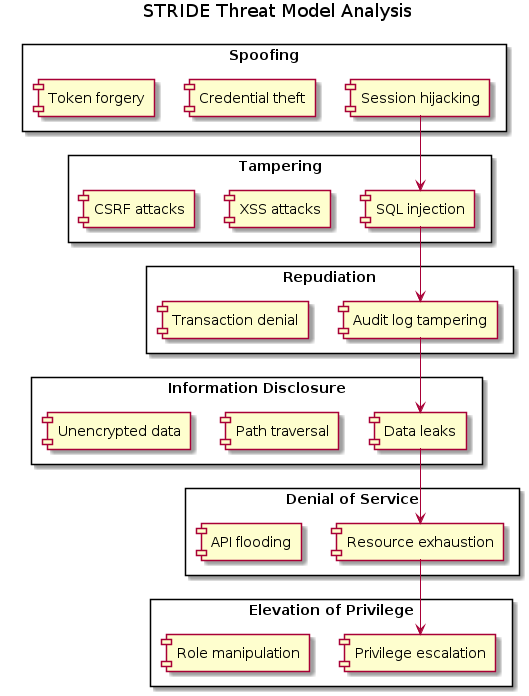
\includegraphics[width=0.7\textwidth]{images/stride-analysis}
	\caption{Visualizing Risk Assessment and Prioritization}
\end{figure}

\subsection*{Reporting Templates}
	extbf{Definition:} Reporting templates standardize the communication of risk findings and recommendations\cite{shostack2014}.
\begin{itemize}
	\item Executive summary
	\item System overview and diagrams
	\item Threat and risk analysis tables
	\item Security control recommendations
	\item Action plan and timeline
\end{itemize}

\subsection*{Continuous Improvement}
	extbf{Definition:} Continuous improvement is the ongoing process of refining security practices based on lessons learned and evolving threats\cite{owasp}.
\begin{itemize}
	\item Integrate threat modeling into DevSecOps pipelines
	\item Schedule regular reviews and updates
	\item Track metrics (e.g., number of threats mitigated, time to remediation)
	\item Foster a security-aware culture through training and awareness
\end{itemize}
